\section{Decision Trees}
\begin{multicols}{2}

Decision trees are a popular supervised learning method that like many other learning methods we've seen, can be used for both regression and classification. Decision trees are easy to use and understand and are often a good exploratory method if you're interested in getting a better idea about what the influential features are in your dataset. 

Basically, decision trees learn a series of explicit if then rules on feature values that result in a decision that predicts the target value. Here's a simple example. Suppose we're playing a game where one person is thinking of one of several possible objects so let's say, an automobile, a bus, an airplane, a bird, an elephant and a dog. 

A second person has to guess the identity of that thing by asking as few yes or no questions as possible up to a limit of no more than say, 10 questions. Suppose the first person secretly thinks of an automobile. So one of the first questions the second person might ask is, "Is it alive?" Intuitively, we know that this type of broad question is much more informative and helps eliminate a larger set of possibilities early on, compared to asking a more specific question right away like, "does it have orange fur with black stripes?" 

The more specific questions might be useful later once we've narrowed the class of things down to particular animals or vehicles, for example. If we think of the property of being alive as a binary feature of an object and the property of having orange fur with black stripes as another feature, we can say that the is a live feature is more informative at an early stage of guessing and thus would appear higher in our tree of questions. When the answer to the first question comes back as "No, it's not alive". 

A second question might be, "Does it fly?" When that answer comes back, no. We can continue to narrow down the set of possible answers by asking more and more specific questions such as, "Can it carry more than 10 people?". In this way any given object can be categorized as either matching the target object the first person is thinking of or not, according to its features as determined by asking the series of yes or no questions. 

We can form these questions into a tree with a node representing one question and the yes or no possible answers as the left and right branches from that node that connect the node to the next level of the tree. One question being answered at each level. At the bottom of the tree are nodes called leaf nodes that represent actual objects as the possible answers. For any object there's a path from the root of the tree to that object that is determined by the answers to the specific yes or no questions at each level. For example a dog is alive cannot fly and doesn't have a trunk. You can view this as a kind of simple decision tree for predicting the class of an object. 

We can generalize this idea of finding a set of rules that can learn to categorize an object into the correct category to many other classification tasks. For example, we're going to look at a classification task next that involves finding rules that can predict what species a particular flower is, based on measurements of certain parts of the flower. 

Rather than try to figure out these rules manually for every task, there are supervised algorithms that can learn them for us in a way that gets to an accurate decision quickly, which we'll look at now. Let's start by looking at a famous dataset in machine learning called the iris dataset. This dataset is included with scikit-learn in the datasets module. Each instance in the dataset represents one of three different species of Iris, a type of flower. 

There are four attributes or features for each instance, that represent measurements of different parts of the flower. The sepal length in centimeters, the sepal width in centimeters, petal length in centimeters and petal width in centimeters. The three species are called setosa, the versicolor and virginica. The data set has measurements for 150 flowers with 50 examples of each species. The classification task is to predict which of the three species and instances given these measurements. Unlike our simple example involving yes or no questions which were binary features of the object. 

The iris data sets features are continuous values. So the rules to be learned will be of the form for example, "Is Petal length greater than 2.3 centimeters?". Let's take a look at how a decision tree is built on this data. The goal when building a decision tree is to find the sequence of questions that has the best accuracy at classifying the data in the fewest steps. Looking at a decision tree, each decision splits the data into two branches based on some feature value being above or below a threshold. For example, whether the petal width is greater than one point two centimeters might be an example of a splitting rule that threshold is called a split point. 

An important concept is \emph{how informative} a split of the data is. So intuitively an informative split of the data is one that does an excellent job at separating one class from the others. 

\begin{center}
	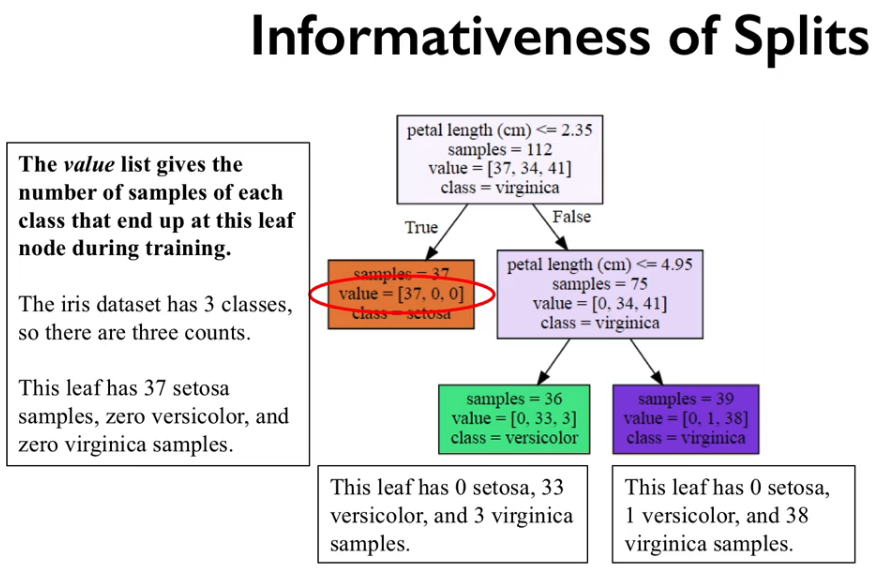
\includegraphics[width=\linewidth]{img/Decision-Tree-Informativeness-of-Splits.png} 
\end{center} 

An example of an informative split might be to put all instances of the flowers with petal length less than 2.35 centimeters into one bin and the rest in the other bin. This is an informative split because at least for this training set, using that rule separates the setosa class completely from the others and allows us to predict the setosa class perfectly just based on this one measurement. A less informative split. 

Like a rule like sepal width less than or equal to three centimeters, would not produce as clear a separation of one class from the others. So for the best split, the results should produce as homogeneous a set of classes as possible. 

There are a number of mathematical ways to compute the best split. One criterion that's widely used for decision trees is called \emph{information gain}, for example. 

So to build the decision tree, the decision tree building algorithm starts by finding the feature that leads to the \emph{most informative} split. 

For any given split of the data on a particular feature value, even for the best split it's likely that some examples will still be incorrectly classified or need further splitting. 

In the iris data set, if we look at all the flowers with petal length greater than 2.35 centimeters for example. Using that split leaves a pool of instances that are a combination of virginica and versicolor that still need to be distinguished further. 

So we can further improve the accuracy of the classification by continuing this process of finding the best split for the remaining subsets with the iris dataset. 

We can further split into flowers that have petal length less than versus greater than 4.95 centimeters for example. This second split is informative because the resulting subsets are more homogeneous that is split did a good job at dividing virginica from versicolor based on the second split test. 

We can continue this process recursively until we're left with leaves in the decision tree that all have the \emph{same} or at least a \emph{predominant majority} of a target value. 

Trees whose leaf nodes each have all the same target value are called \emph{pure}, as opposed to \emph{mixed} where the leaf nodes are allowed to contain at least some mixture of the classes. 

To predict the class of a new instance given its feature measurements, using the decision tree we simply start at the root of the decision tree and take the decision at each level based on the appropriate feature measurement until we get to a leafnode. The prediction is then just the majority class of the instances in that leafnode. 

\begin{center}
	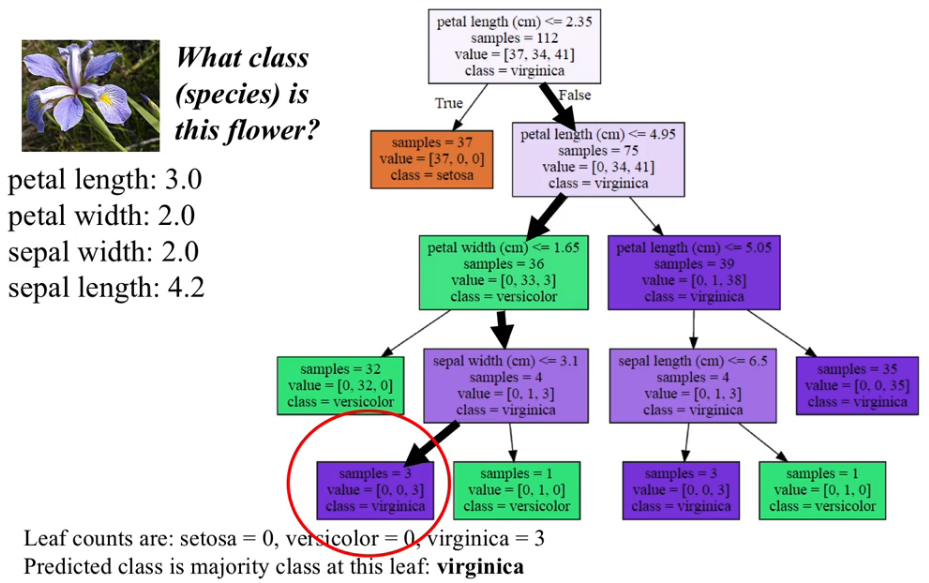
\includegraphics[width=\linewidth]{img/Decision-Tree-2.png} 
\end{center} 


So for the iris data for example, a flower that has a petal length of three centimeters, a petal width of two centimeters and a sepal width of two centimeters would end up at this leafnode, whose instances are all of the virginica class. So the prediction would be virginica. 

\subsection{Regression}

Decision trees can also be used for regression using the same process of testing the future values at each node and predicting the target value based on the contents of the leafnode. For regression, the leafnode prediction would be the mean value of the target values for the training points in that leaf. 

\subsection{Implementation}

In scikit-learn, to build the decision tree you import the Decision tree classifier class from the scikit-learn tree module and fit it just as you would any classifier by creating the object and calling the fit method on the training data. 

{\scriptsize
\begin{verbatim}
from sklearn.tree import DecisionTreeClassifier
...
Accuracy of Decision Tree classifier on training set: 1.00
Accuracy of Decision Tree classifier on test set:     0.95
\end{verbatim}
}

\subsection{Overfitting Control}

Notice that the training data here is predicted perfectly with an accuracy of 1.0. While the test data is a little bit worse. This is an indication that the tree is likely \emph{overfitting} and in fact this is a problem with building decision trees in general that keep adding rules until the leafnodes are pure. 

Typically such trees are \emph{overly complex and essentially memorized the training data}. So when building decision trees, we need to use some additional strategy to prevent this overfitting. One strategy to prevent overfitting is to prevent the tree from becoming really detailed and complex by stopping its growth early. This is called \emph{pre-pruning}. 

Another strategy is to build a complete tree with pure leaves but then to prune back the tree into a simpler form. This is called \emph{post-pruning} or sometimes just pruning. The decision tree implementation and \texttt{scikit-learn} only implements \emph{pre-pruning}. 

We can control tree complexity via \emph{pruning} by limiting either the maximum depth of the tree using the \texttt{max_depth} parameter or the maximum number of leafnodes using the \texttt{max_leafnodes} parameter. We could also set a threshold on the minimum number of instances that must be in a node to consider splitting it. And this would be using the \texttt{min_samples_leaf} parameter. 

We can see the effect of pre-pruning by setting \texttt{max_depth = 3} on the iris dataset. Now the accuracy on the training data is slightly worse but the accuracy on the test data is slightly better. 


\end{multicols}
\begin{center}
	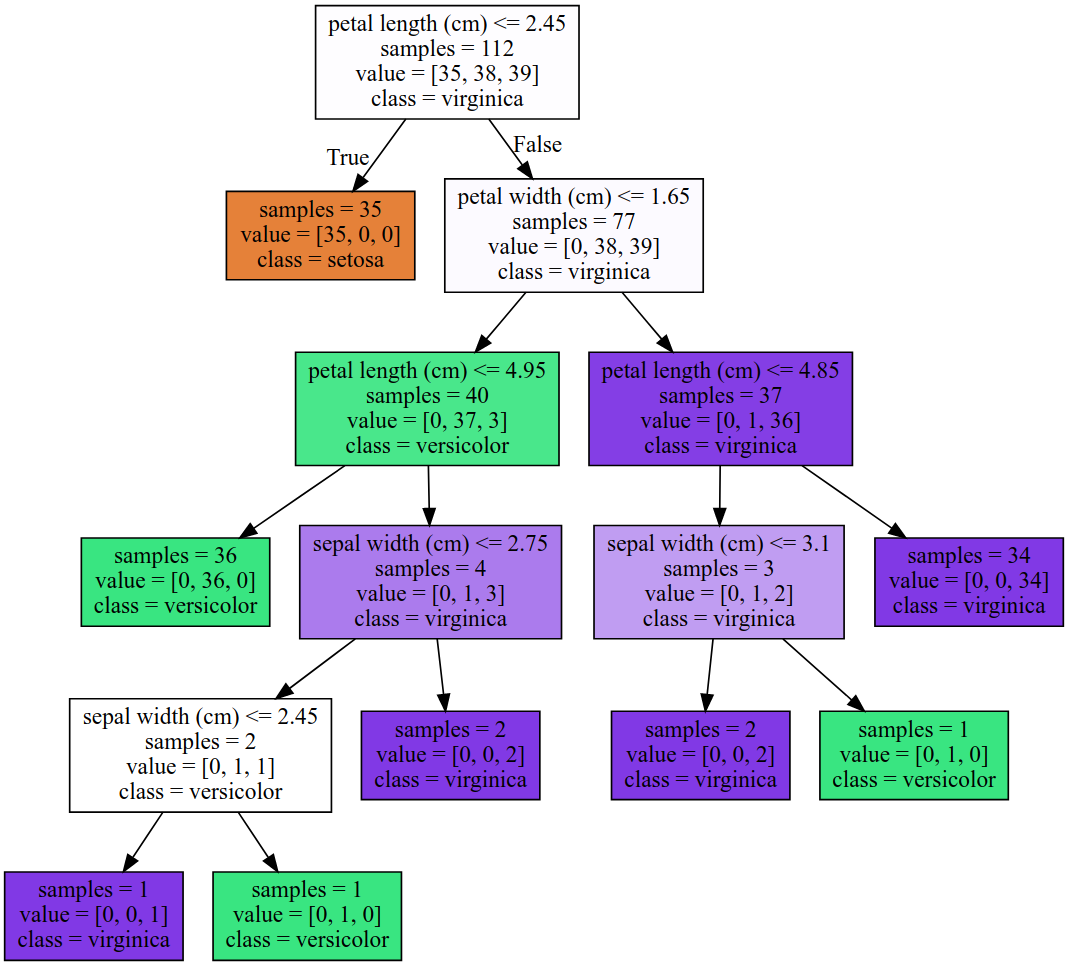
\includegraphics[width=\linewidth]{img/Decision-Tree-3.png} 
\end{center}
\begin{multicols}{2}

\subsection{Visualizing Decision Trees}

One great \textbf{advantage} of decision trees at least for the not too big, is that they're \emph{easy to interpret}. Visualizing the entire tree can show you exactly how did the decision tree is making its predictions. 

So let's take a look at an example. In the \texttt{adspy_shared_utilities.py} we've provided a function call named \texttt{plot_decision_tree} that takes the classifier object, the feature names, and the class names as input. And uses the \texttt{graphviz} library to visualize the tree. It works by calling the export graph its function in the \texttt{scikit-learn.tree} module to create a \texttt{.dot} file which is a text file description of the tree, and then using the \texttt{graphviz} library to visualize the \texttt{.dot}  file creating an image. 

Here's the resulting plot for the unpruned Iris dataset tree.The first line in a node indicates the decision rule being applied for that node. The second line indicates the total number of data instances for that node. The third line shows the class distribution among those instances. And the fourth line shows the majority class of that nodes data instances. For example in the root node the initial pool of data has 37 setosa examples, 34 versicolor examples, and 41 virginica examples. After the first split into subsets that have petal length less than or equal to 2.35 on the left and those that have petal length greater than 2.35 on the right, we have a leafnode on the left that consists entirely of the 37 setosa examples and a decision note on the right that has 34 versicolor and 41 virginica examples. This node on the right then makes a second split based on petal length using a threshold of 4.95 centimeters and that creates two subsets of 36 samples on the left containing 33 versicolor examples and 39 samples on the right, 38 of which are virginica examples. 

We've used an option when plotting the decision tree to fill the nodes with colors that indicate the majority class of the data instances associated with that node. The intensity of the color indicates the strength of the majority count for that class. 

For larger trees that have say a depth of more than 5 or 10. Instead of trying to analyze all the paths in the tree it can be useful to see which paths most of the data takes. This can be done by looking for the largest samples values in the nodes. For example if we follow the largest samples values down this tree, we can see that a significant set of 35 virginica examples are classified perfectly when their petal length is greater than 5.05 centimeters. 

\subsection{Feature Importance}

Another way of analyzing the tree instead of looking at the whole tree at once is to do what's called a \emph{feature importance} calculation. And this is one of the most useful and widely used types of summary analysis you can perform on a supervised learning model. 

Feature importance is typically a number between 0 and 1 that's assigned to an individual feature. It indicates how important that feature is to the overall prediction accuracy. A feature importance of \textbf{0} means that the feature is \emph{not used} at all in the prediction. A feature importance of \textbf{1} means the feature \emph{perfectly predicts} the target. 

Typically, feature importance numbers are \emph{always positive }and they're \emph{normalized} so they sum to one. In \texttt{scikit-learn}, feature importance values are stored as a list in an estimated property called \texttt{feature_importances_}. And note the underscore at the end of the name which indicates it's a property of the object that's set as a result of fitting the model and not say as a user defined property. 

The shared utilities python file contains a function called \texttt{plot_feature_importances}, that you can import and use to visualize future importance. It plots a horizontal bar chart with the features listed along the \texttt{y_axis} by name and feature importance along the \texttt{x_axis}. 

\begin{center}
	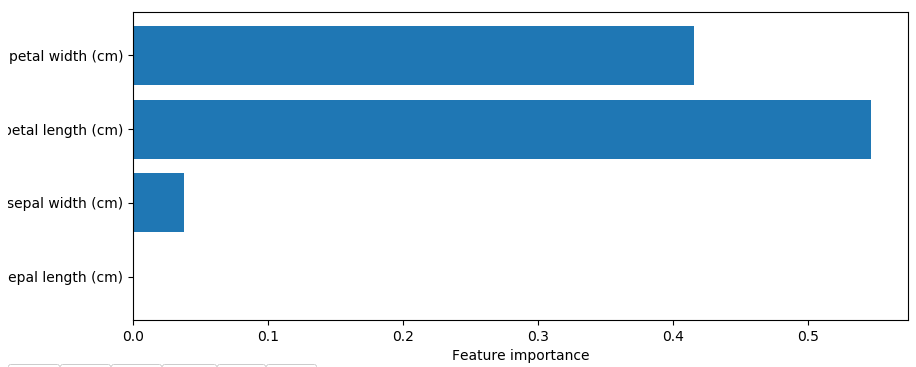
\includegraphics[width=\linewidth]{img/Decision-Tree-Feature-Importance.png} 
\end{center}

Here's the feature importance chart for the iris decision tree and this example for this particular train/test split of the iris data set. The pedal length feature easily has the largest feature importance weight. We can confirm this by looking at the decision tree that this is indeed corresponds to that features position at the top of the decision tree, showing that this first level just using the petal length feature does a good job splitting the turning data into separate classes. 

Note that if a feature has a low feature importance value, that doesn't necessarily mean that the feature is not important for prediction. It simply means that the particular feature wasn't chosen at an early level of the tree and this could be because the future may be identical or highly correlated with another informative feature and so doesn't provide any new additional signal for prediction. Feature importance values don't tell us which specific classes a feature might be especially predictive for, and they also don't indicate more complex relationships between features that may influence prediction. 

Even so the feature importance values provide an easy to understand summary that can give \emph{useful insight} about individual features in the learning model. Because feature importance can vary depending on the specific model learned for a particular train/test split for example. It's common when computing feature importance to use an average over multiple train/test splits. For example when performing cross-validation. 

Finally let's apply decision trees to the breast cancer data set that we've been using across multiple supervised learning algorithms. Here we're controlling them all the complexity by setting the max depth and min samples leaf parameters. And we've included the visualization of the resulting tree here followed by a feature importance plot. 

As an exercise, try removing these two parameters to just use the default settings to see the effect on test set accuracy and the increase in overfitting that occurs. 

For this training set, the mean concave points feature gives the most informative initial split, followed by the worst area parameter. 

\subsection{Pros and Cons}

One of the major advantages of decision trees as a supervised learning method, is that the decision rules are \emph{easily visualized and interpreted} by people including users without machine learning expertise.
This makes decision trees a useful choice for getting an initial understanding of what some of the more important features are likely to be for a particular prediction task. 

Another advantage of decision trees is that you can use them \emph{without} having to do feature pre-processing or \emph{normalization}. Since each feature is processed independently and the splitting of the data doesn't depend on the absolute scale of the feature. The decision algorithm can operate on the original training data pretty much as is. 

So decision trees tend to work well with data sets that have a \emph{mixture of feature types}~--- binary, categorical or continuous and with features that are on very different scales. 

One \textbf{drawback} of decision trees is that despite the use of pruning they can still \emph{overfit} all or parts of the data and \emph{may not achieve the best generalization performance} compared to other methods. 

One way to overcome that problem is to create what's called an \emph{ensemble of decision trees} which combines multiple decision trees to make a prediction and will look at ensembles of decision trees in the following lecture. 

So to recap, scikit-learn enables you to control the model complexity of your decision trees with three key parameters. First, \texttt{max_depth} controls the maximum depth or the number of split points the decision can have and it's probably the most common parameter used to reduce tree complexity and thus reduce overfitting. The \texttt{min_samples_leaf}  parameter is the threshold that controls what the minimum number of data instances has to be in a leaf to avoid splitting it further. This setting also reduces tree complexity. Finally, \texttt{max_leaf_nodes} limits the total number of nodes that are leaves of the tree. 

In effect, setting this parameter will indirectly influence the other two parameters and vice versa. So in practice, adjusting only one of these trees is typically enough to control most overfitting. Although even with the most optimized parameter settings, individual decision trees will still tend to overfit. 
\end{multicols}